\documentclass[letterpaper]{jdf}
\usepackage{graphicx,booktabs,array,hyperref}
\author{Zihan Zheng}
\email{zzheng399@gatech.edu}
\title{Individual Project Check-In 3: Evaluation Plan for Safer Email Sending and Recovery}
\begin{document}
\maketitle
\section{Project Overview and Status}
This project focuses on the existing task of sending an email accurately and responding to errors around the Send action, not redesigning a whole email client. Check-In 1 documented an unsuccessful attempt to Recall a message sent from Outlook to an external Gmail account. Check-In 2 reported an 18-person convenience survey (including 15 reporting forgotten attachments and 10 selecting wrong recipients), brainstorming, and three low-fidelity designs. These observations motivate the designs but are not population-wide claims. No first-round participant evaluation has yet been conducted.

Prototype A (Pre-Send Safety Check) warns about a likely missing attachment, then allows correction or override. Prototype B (Delayed Send and Undo) displays a pending-send countdown during which an incorrect send can be cancelled. Prototype C (Transparent Recovery Assistant) explains the limits of recalling an already delivered external email and supports realistic follow-up. These are proposed interactions, not verified Outlook features. The three storyboard files are retained in the repository. This check-in solicits feedback on the initial evaluation plan.

\begin{figure}[ht]\centering
\begingroup\scriptsize\setlength{\fboxsep}{5pt}
\fbox{\begin{minipage}{.27\linewidth}\textbf{1. Compose}\\[3pt]\hrule\smallskip
To: professor@school.edu\\Subject: Project report\\[4pt]
Please see attached report.\\[6pt]\fbox{Send}
\end{minipage}}\hfill$\rightarrow$\hfill
\fbox{\begin{minipage}{.27\linewidth}\textbf{2. Check}\\[3pt]\hrule\smallskip
\textbf{No attachment found}\\[3pt]
Did you forget a file?\\[5pt]\fbox{Go back}
\end{minipage}}\hfill$\rightarrow$\hfill
\fbox{\begin{minipage}{.27\linewidth}\textbf{3. Revise}\\[3pt]\hrule\smallskip
To: professor@school.edu\\Subject: Project report\\[4pt]
Attachment: report.pdf\\[6pt]\fbox{Send}
\end{minipage}}\endgroup
\caption{Prototype A: targeted pre-send warning and draft correction.}
\end{figure}
\begin{figure}[ht]\centering
% Vector source and PNG preview: Figures/render_prototypes.py
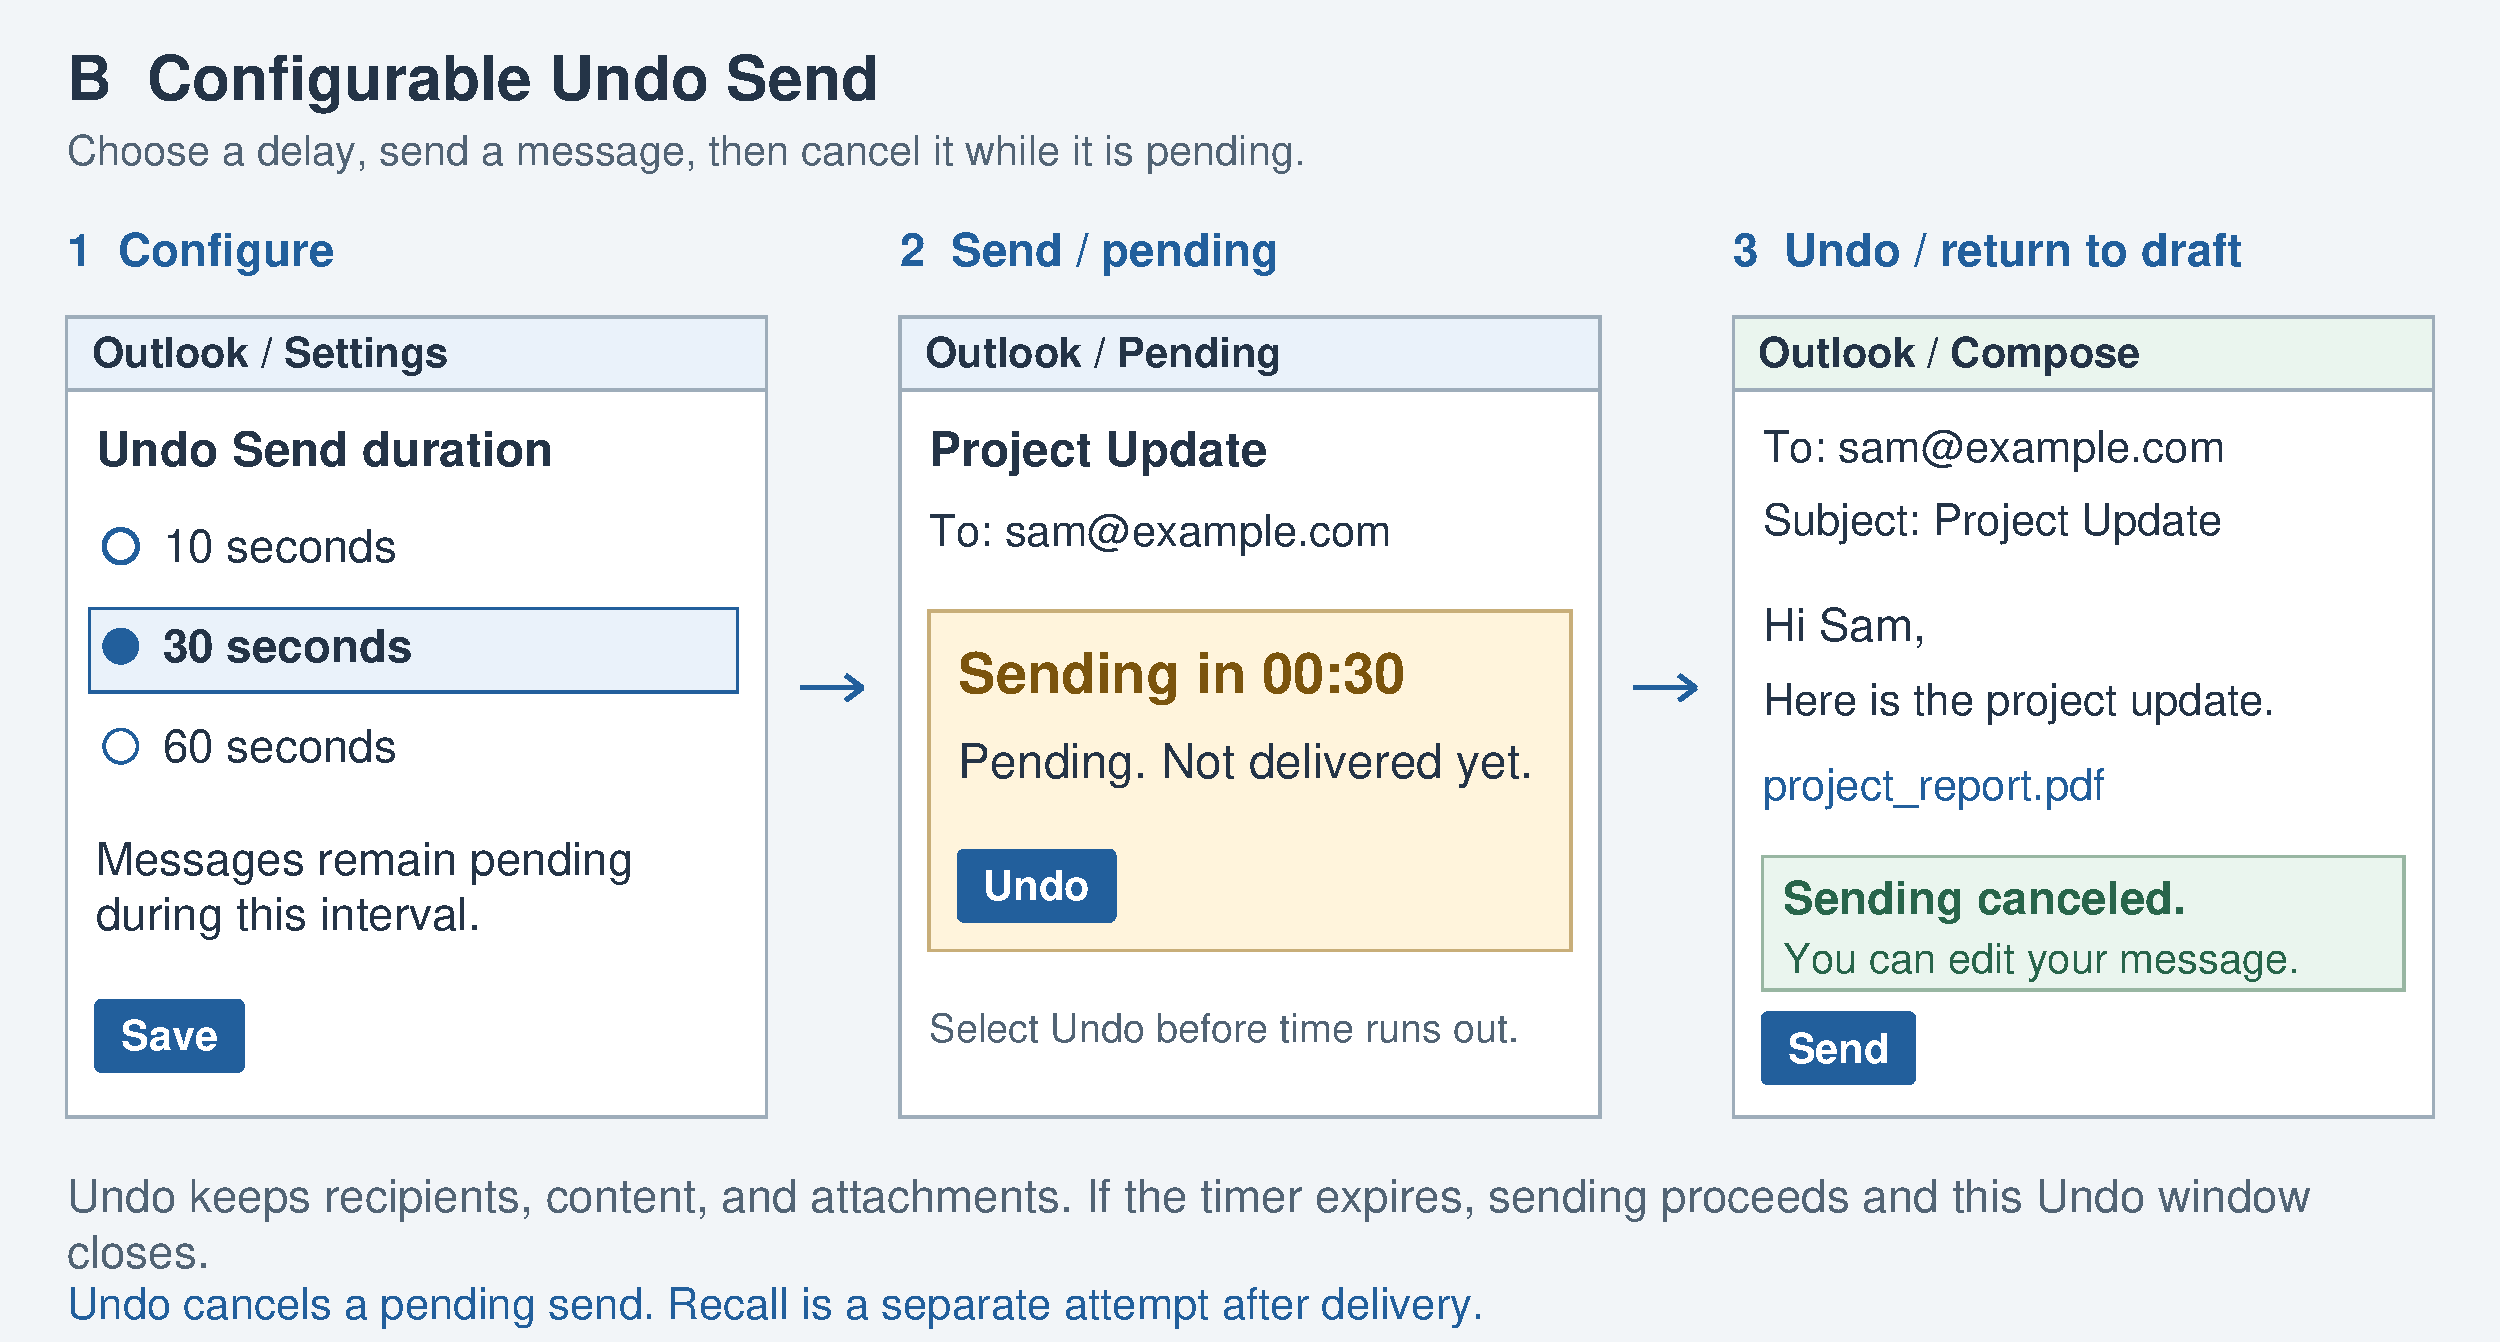
\includegraphics[width=\linewidth,page=1]{Figures/prototype_b.pdf}

\caption{Prototype B: delayed send, visible Undo window, and cancellation.}
\end{figure}
\begin{figure}[ht]\centering
\begingroup\scriptsize\setlength{\fboxsep}{5pt}
\fbox{\begin{minipage}{.27\linewidth}\textbf{1. Message}\\[3pt]\hrule\smallskip
To: external@gmail.com\\Subject: Project report\\[5pt]
\textbf{Delivered}\\[5pt]\fbox{Recovery}
\end{minipage}}\hfill$\rightarrow$\hfill
\fbox{\begin{minipage}{.27\linewidth}\textbf{2. Explanation}\\[3pt]\hrule\smallskip
\textbf{Recall unavailable}\\[3pt]External delivery cannot be undone by Recall.
\end{minipage}}\hfill$\rightarrow$\hfill
\fbox{\begin{minipage}{.27\linewidth}\textbf{3. Recovery}\\[3pt]\hrule\smallskip
\textbf{Next steps}\\[4pt]\fbox{Send correction}\\[5pt]\fbox{Contact recipient}
\end{minipage}}\endgroup
\caption{Prototype C: transparent status and corrective follow-up.}
\end{figure}

\section{Objectives and Comparison Strategy}
The evaluation asks: (1) Can users understand each system state and their next action? (2) Can users respond appropriately to each sending mistake? (3) Which safeguards are useful or disruptive, and why? Each participant will examine all three prototypes. Shared ratings will support comparison of perceived clarity, ease, confidence, and usefulness across A/B/C. Because the scenarios represent different stages of sending, task success rates will be interpreted separately within each scenario, not used to rank A/B/C as if tasks were identical. Feedback will inform the selection or combination of features for the second-iteration medium-fidelity prototype.

\section{Participants, Recruitment, and Materials}
The target is 5--6 adult, regular email users, recruited from classmates and acquaintances, ideally with varied Gmail/Outlook experience. Invitations will describe an approximately 15--20 minute voluntary session with fictional emails. Participation credit will be mentioned only if actually available through course procedures; no incentive is guaranteed. No real messages will be sent, and no login details or identifying raw survey exports will be collected. Each person will review all three paper-style storyboards. A facilitator advances to the next state in response to the participant's selection; this is a facilitator-operated paper prototype, not functional software. Prototype order will vary across participants (ABC, BCA, CAB) to limit sequence effects. Participants can skip questions or stop. Notes use anonymous identifiers (P01, etc.).

\section{Evaluation Procedure}
\begin{enumerate}
\item \textbf{Opening (2 minutes):} Explain the purpose, confirm voluntary participation and consent to anonymous note-taking, and state that the interface, not the participant, is being tested.
\item \textbf{Background (2 minutes):} Ask which email client the participant usually uses, frequency of use, and familiarity with Undo Send and Recall.
\item \textbf{Tasks (9--12 minutes including ratings):} For each prototype, read the corresponding prompt in Table 1 without revealing the correct action. Ask the participant to think aloud and point to or describe a chosen action. Show the resulting storyboard state. Record completion without/with help or failure, incorrect actions, misunderstandings, and comments. Use only neutral prompts if stuck and record any assistance.
\item \textbf{Post-task ratings:} After each prototype, ask the four identical five-point questions in Appendix B.
\item \textbf{Wrap-up (2 minutes):} Ask for overall preference, concerns, and desired changes; thank the participant.
\end{enumerate}
\begin{table}[ht]\centering\small
\begin{tabular}{p{.12\linewidth}p{.43\linewidth}p{.34\linewidth}}\toprule
Design & Fictional task & Suitable response\\\midrule
A & You tell a professor a report is attached, forget the attachment, and press Send. What do you do? & Notice the warning and add the attachment before sending (or explain a valid override).\\
B & Just after pressing Send, you realize the recipient is wrong. What do you do? & Use Undo before the pending countdown expires, then correct the draft.\\
C & You discover an inaccurate message was already delivered to an external Gmail recipient. What now? & Acknowledge no guaranteed recall of delivered mail; choose a realistic follow-up such as a correction.\\\bottomrule
\end{tabular}
\caption{Scenarios and prototype-specific success criteria.}
\end{table}

\section{Quantitative and Qualitative Measures}
\subsection{Numerical measures and planned statistical analysis}
After each scenario, collect four common 1--5 Likert ratings: Q1, understanding the system state; Q2, knowing the next action; Q3, confidence in handling the mistake; Q4, usefulness in routine emailing. Record completion (without help / with help / not completed) and number of erroneous actions as additional diagnostic counts. Summarize each rating by prototype using median, range, and response distribution; report task outcome and error counts by task.

The preselected primary comparative outcome is Q1 (clarity). Since the same 5--6 participants rate all three alternatives on an ordinal scale, perform a Friedman repeated-measures test for Q1, reporting test statistic and p-value. Treat the other ratings descriptively to avoid inflating multiple-testing claims. If missing responses prevent meaningful matched analysis, state the limitation and present descriptive results rather than manufacture inferential statistics. A non-significant result in this small, low-powered sample will not be interpreted as proof of equivalent designs. The numeric comparison concerns user perceptions, not relative task success across non-equivalent scenarios.

\subsection{Qualitative questions and analysis}
Ask participants to think aloud during tasks. After each, ask what was confusing and what they would change. At the end, ask which safeguard they prefer and why; inquire about interruptions, privacy, and misleading expectations. Summarize anonymized comments and categorize by themes, initially including warning fatigue, timer visibility, Undo/Recall misunderstanding, and recovery trust while allowing new categories. Report the count of participants mentioning each theme and concise illustrative paraphrases. These are potential coding themes, not observed findings.

\section{Planned Use of Findings}
The first evaluation will identify usability issues and guide a documented second-iteration design decision. For example, if users miss the countdown, make the pending state more prominent; if they misinterpret Recall, clarify delivery status; if warnings are intrusive, narrow trigger conditions. These are contingent decisions rather than asserted results. The final report will separately document actual recruitment, deviations from plan, numeric findings and statistical results, qualitative themes, and design revisions.

\section{Peer Feedback Requested}
Are the three task prompts clear and neutral? Is the cross-prototype rating comparison appropriate despite different error stages? What interface states or potential misunderstandings are missing? Is this participant and analysis plan feasible?

\appendix
\section{Facilitator Script}
Opening: Thank you for helping evaluate three early ideas for addressing email-sending mistakes. This is a test of the interfaces, not you. The emails are fictional. Please explain what you think is happening and point to the action you would take. I will advance the mock interface based on your choice. May I take de-identified notes? You can stop at any time.

For each prototype: Read the matching Table 1 prompt. Ask: What do you expect to happen? What would you do next? Show the next paper state only after the response. If the participant is stuck, record it before asking a neutral question such as: What options do you see?

Close: Which approach would you want in your everyday email client, and why? What trade-off worries you? What one change would you make?

\section{Complete Evaluation Questions}
Background: (1) Which email service do you use most? (2) How often do you send email? (3) Have you used Undo Send or Recall?

After \emph{each} A, B, C, circle a rating from 1 (strongly disagree) to 5 (strongly agree):
\begin{enumerate}
\item I understood what the system was doing.
\item I knew what action to take next.
\item I felt confident handling the mistake.
\item I would find this safeguard useful when sending email.
\end{enumerate}
Open-ended: What was confusing? What would you change?

After all three: Which safeguard do you prefer for routine email and why? Which feels intrusive or misleading? Do you have concerns about privacy or delay?

\section{Blank Evaluation Recording Sheet}
\begin{table}[ht]\centering\small
\begin{tabular}{p{.09\linewidth}p{.12\linewidth}ccccp{.24\linewidth}}\toprule
ID & Design & Q1 & Q2 & Q3 & Q4 & Task outcome / errors / notes\\\midrule
P01 & A & -- & -- & -- & -- & Not collected\\
P01 & B & -- & -- & -- & -- & Not collected\\
P01 & C & -- & -- & -- & -- & Not collected\\
P02--06 & A/B/C & -- & -- & -- & -- & Add after sessions\\\bottomrule
\end{tabular}
\caption{Empty data structure only; no evaluation results are implied.}
\end{table}

\section{Final Assignment Requirements Still Outstanding}
This check-in is not the complete final report. The November 9 individual project requires: documenting actual first-round evaluation results with the planned quantitative test and qualitative analysis; second-iteration planning; a medium-fidelity prototype; an accessible approximately five-minute video walkthrough with narration and design rationale; a separate final evaluation plan; and actual final evaluation results with quantitative and qualitative analysis. The earlier required heuristic evaluation of an existing email interface using at least three heuristics still needs documented execution and findings; Check-In 2 explicitly noted this gap. Relevant raw instruments/results and any AI-assisted brainstorming transcript belong in final appendices. The final JDF PDF must be composed in Overleaf, with its edit-share link submitted as required. These pending tasks are not represented as completed.
\end{document}

